\section{Anwendersicht}
Für die Anwendersicht wurden zwei Applikationen erstellt. Zum einen eine Mobile Applikation und zum anderen eine Web Applikation. Die Mobile Applikation wurde für das Betriebssystem Android in AndroidStudio entwickelt. Die Web Applikation wurde mit Hilfe eines Bootstrap Templates erstellt. Beide Applikationen verwenden die Bibliothek Paho um mit der MOM zu Interagieren.  
\subsection{Andriod-APP}
Die Android Applikation soll eine Wetter Applikation sein, dafür soll sie verschiedene Wetterdaten anzeigen können. Dazu wurde zu beginn des Projektes festgelegt, welche Daten anzeigt werden  sollen. Diese können in zwei Kategorien unterschieden werden. Zum einen das \textbf{Tageswetter} und zum anderen die \textbf{Wochenvorhersage}. Unter das Tageswetter fallen die folgenden Punkte: 
\begin{itemize}
\item das Tageswetter als großes Icon
\item die momentane Temperatur in $^\circ$C
\item das genaue Wetter in Wörtern
\item der Standort
\item das Datum mit Uhrzeit
\item die Windgeschwindigkeit in km/h
\item die Windrichtung mit Hilfe einer grafischen Anzeige
\item die Regenwahrscheinlichkeit in \%
\end{itemize}  
Bei der Wettervorhersage für eine Woche ergeben sich nachfolgende Punkte
\begin{itemize}
\item die Wochentage ab dem nachfolge Tag des Tageswetters
\item ein kleines Wettericon
\item die Tagesmaximaltemperatur in $^\circ$C mit der Schriftfarbe rot
\item die Tagesminimaltemperatur in $^\circ$C mit der Schriftfarbe blau
\item ein Diagramm das die Maximal- und Minimaltemperaturen veranschaulicht
\end{itemize}  
Des Weiteren sollte es eine Auswahlmöglichkeit geben zwischen der Automatischen Standortbestimmung mittels GPS und der Eingabe einer Postleitzahl um den Standort festzulegen.
\begin{figure}[htbp]
	\centering
	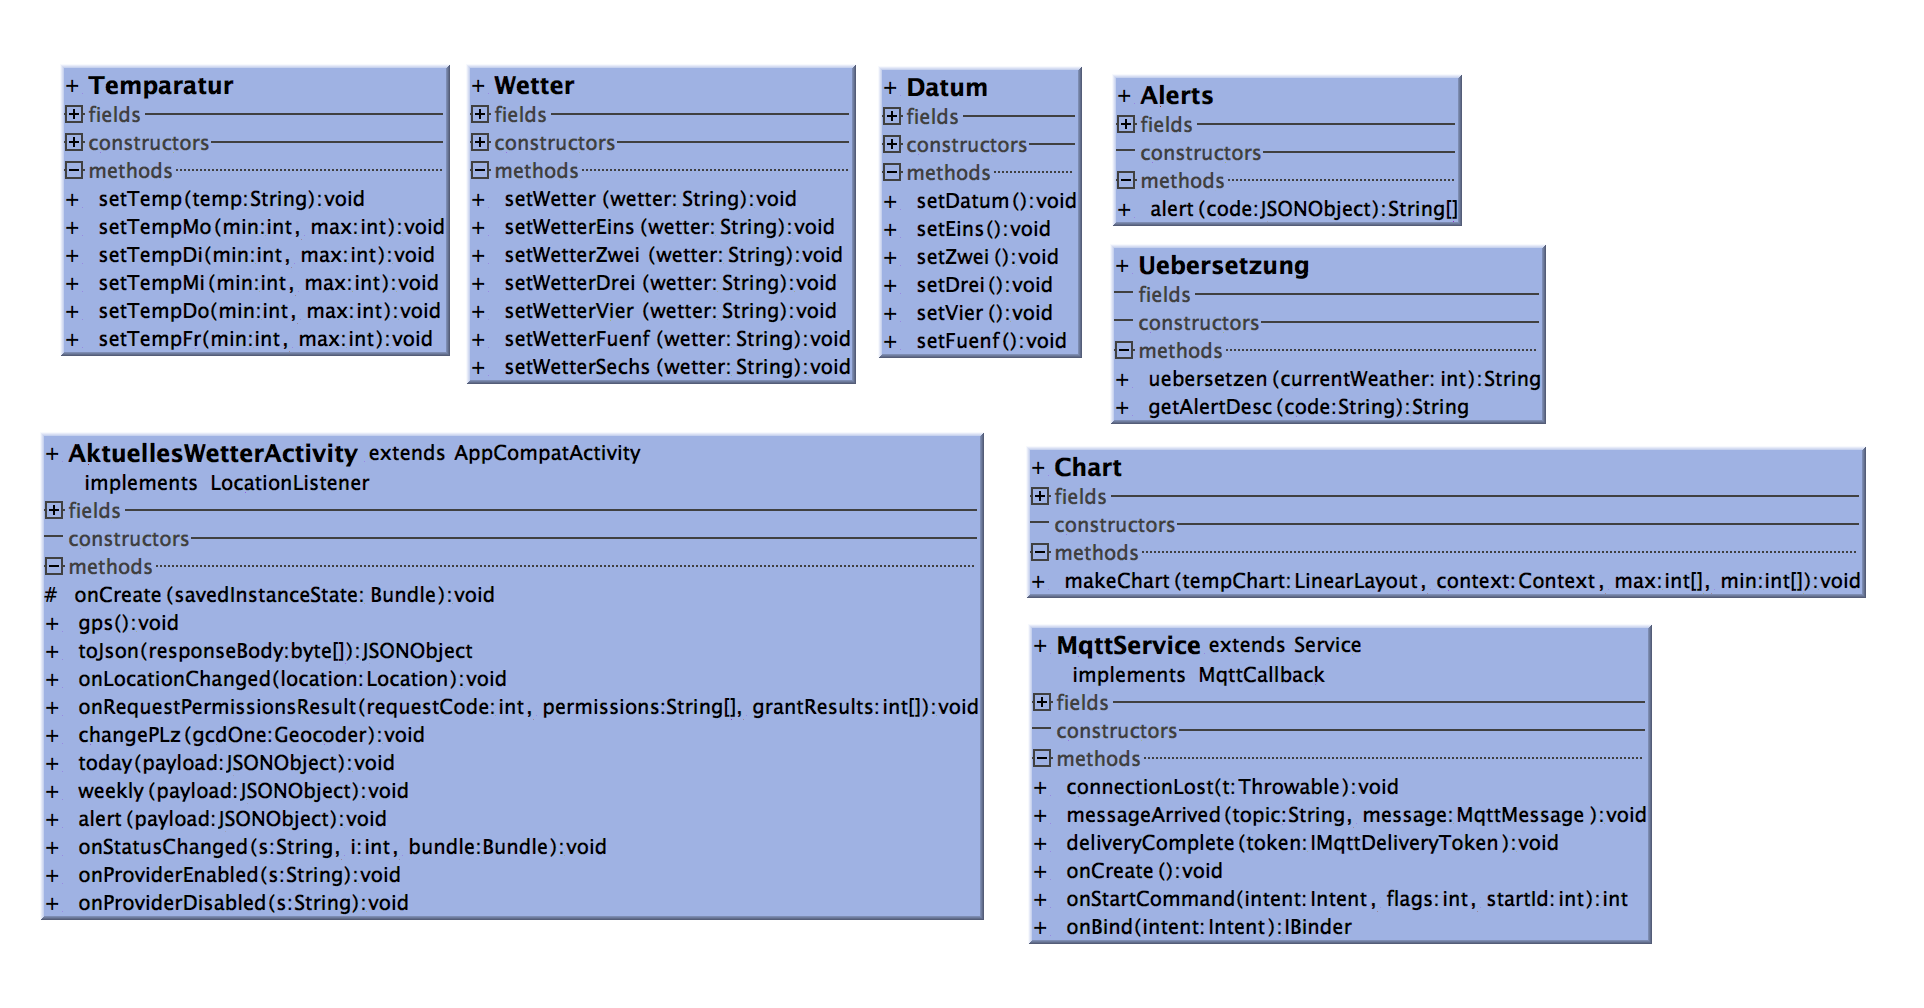
\includegraphics[width=1.0\textwidth]{Bilder/AndroidUML.png}
	\caption{Klassendiagramm der Android-Applikation}
	\label{img:AndroidUMLDiagramm}
\end{figure} 
Die Applikation wurde in Androidstudio in der Sprache Java und XML geschrieben. 
Aufgebaut ist die Applikation über 8 Klassen wie in  Abb. \ref{img:AndroidUMLDiagramm} zusehen ist. Die Klasse \textbf{AktuellesWetterActivity} fungiert dabei als Main-Class.
Die Klasse \textbf{MqttService} ist ein Android Service. Als einen Android Service bezeichnet man einen Prozess der Nebenläufig zum Hauptprozess läuft. Dieser Service ist für die Verbindung zur MoM notwendig und wird später in Unterkapitel \ref{subsubsec:MqttService} näher erläutert.
Die Weiteren Klassen sind Hilfsklassen zur Verarbeitung der, durch die MoM bereitgestellten Daten.
So zum Beispiel übersetzt die Klasse \textbf{Uebersetzung} die verschiedenen Wettercodes, in für den Anwender lesbare Wetterbezeichnungen. Dies geschieht mit Hilfe einer einfachen Switch-Case-Anweisung wie exemplarisch in Abb. \ref{img:Case-Uebersetzung} zu sehen.
  \begin{lstlisting}
 switch (code) {
            case "H1": {
                return "Starke Luftdruckschwankungen, nehmen Sie Ihre Medizin falls benoetigt";
            }
            case "H2": {
                return "Temperaturen ueber 25 $^\circ$C, nehmen Sie Ihre Medizin falls benoetigt";
            }
            case "S1": {
                return "Ideales Badewetter";
            }
            case "W1": {
                return "Achtung, Frostgefahr";
            }
            case "W2": {
                return "Achtung, sehr niedrige Temperaturen. Ziehen Sie sich warm an.";
            }
            case "W3": {
                return "Achtung, schwere Schneefaelle.";
            }
            case "T1": {
                return "Luftfeuchtigkeit ueber 90%";
            }
        }
	\label{img:Case-Uebersetzung}
\end{lstlisting} 

Bei beginn der Applikation soll wie in den Anforderungen beschreiben die Position automatisch durch GPS ermittelt werden. Dazu wurde das von Android bereitgestellte Interface LocationListener verwendet. Dazu müssen die Methoden onLocationChanged(), onProviderDisabled(), onProviderEnabled() und onStatusChanged() implementiert werden. 
Die wichtigste Methode dabei ist die onLocationChanged(). Diese liefert jedes Mal wenn sich die Position des Smartphones verändert die neue Position zurück. 
Um nun das Interface LocationListener zu verwenden ist es notwendig sich den Location Service bei den SystemServices zu holen die geschieht über folgende Codezeile:
  \begin{lstlisting}
   LocationManager locationManager = (LocationManager) getSystemService(Context.LOCATION_SERVICE);
  \end{lstlisting}
  Des Weiteren ist es notwendig ab Android Version 6.0 (API level 23) dem Anwender die Möglichkeit zugeben die Standortbestimmung mittels GPS zu verweigern. Dafür muss eine Permissions Abfrage gemacht werden, diese wird von Android fertig geliefert und muss nur in den Code eingebaut werden. Wenn das geschehen ist kann über das Objekt locationManager die Methode requestLocationUpdates(String provider,long minTime, float minDistance, LocationListener listener) mit den Parametern: 
    \begin{itemize}
\item provider = "gps"
\item minTime = 10000 (Millisekunden)(dieser Wert ist für die App nicht so wichtig, da die Aktualisierung nur beim Start und auf Knopfdruck benötigt wird)
\item minDistance = 50 (in Meter)(dieser Wert ist für diese App nicht so wichtig, da die Genauigkeit der Position eine untergeordnete Rolle spielt)
\item listener = this (Klasse die das Interface LocationListener implementiert)
\end{itemize}  
aufrufen. Nach dem diese Methode mit den Settings des LocationManagers aufgerufen wurde kann die Methode getLastKnownLocation("gps") der Klasse LocationManager aufgerufen werden. Diese Methode Liefert ein Objekt der Klasse Location zurück. Dieses Location Objekt beinhaltet die Positionsdaten. Um nun von den Positionsdaten auf die benötigten angaben wie Stadtnamen und Postleitzahl (PLZ) zukommen, wird ein Objekt der Klasse Geocoder benötigt. Die Klasse Geocoder ist ebenfalls Bestandteil der Android Location Library. Durch diese Klasse können die Längen- und Breitengrad Daten des Location Objektes in Stadtnamen und PLZ umgewandelt werden.
Liegen diese Daten vor kann der Stadtname auf der App angezeigt werden und der Android Service MqttService mit dem Übergabeparameter PLZ über folgenden Code 
 \begin{lstlisting}
private Intent serv = new Intent(this, MqttService.class);
serv.putExtra("plz", plz); 
startService(serv);
  \end{lstlisting}
gestartet werden.
\subsubsection{Mqtt Service}
\label{subsubsec:MqttService}
Der MqttService ist das Herzstück der Android Applikation in diesem Service wird die Verbindung zur MOM hergestellt und die Daten die diese liefert Empfangen.
Mit dem Open Source Projekt Paho wurde eine Verbindung zu der in Kapitel \ref{rabbitmq} vorgestellten MOM realisiert. Dafür wurde die für Android spezifische Library über Grovy importiert. Durch diesen Import ist es möglich einen Android-Client zu erstellen. Dafür wurde das Interface MqttCallback implementiert. Zu diesem Interface gehören die Methoden: 
 \begin{itemize}
\item connectionLost(Throwable t):
\\Diese Methode hat den Zweck, wenn während des Betriebs der Applikation die Verbindung zur MOM verloren geht, diese wieder aufzubauen.
\item messageArrived(String topic, MqttMessage message):
\\In dieser Methode kommen die Messages der Abonnierten Topics als Byte Arrays und das dazugehörige Topic als String, zur Unterscheidung der Messages an.
\item deliveryComplete(IMqttDeliveryToken token):
\\Wird aufgerufen, wenn die Zustellung für eine Nachricht abgeschlossen ist und alle Bestätigungen eingegangen sind.
\end{itemize}
Wie im vorherigen Kapitel erwähnt wird der Service mit dem Parameter PLZ gestartet, dazu wird die Methode onStartCommand verwendet, diese besitzt als Aufrufparameter ein Intentobjekt, diesem wurde in der AktuellesWetterActivity ein "Extra" mit dem Key plz übergeben. Mit Hilfe dieses Keys kann der Übergebene Wert ausgelesen werden. Um nun eine Verbindung mit der MOM aufzubauen, werden vier Angaben benötigt. Diese sind zum einen die tcp-url und der Port der MOM. Zum anderen für die Authentifizierung bei der MOM einen Usernamen und ein Passwort. Der Username und das Passwort werden einem Paho ConnectionOption Objekt übergeben. Dabei wird das Passwort mittels eines Char-Arrays übergeben. Dieses ConnectionOption Objekt wird wiederum zusammen mit der Url, dem Port und einer Client-Id (diese wird automatisch erzeugt) an das eigentlichen Client Objekt übergeben. Dieses Client Objekt besitzt die Methode connect in dieser wird das Interface IMqttActionListener mit den Methoden onSuccess und onFailure aufgerufen. In der Methode onSuccess werden nun 3 Topics der MOM abonniert. Diese 3 Topics sind:
\begin{itemize}
\item plz/today/CEP:
\\ Liefert ein JSON Objekt mit dem Tages aktuellen Wetter für die Postleitzahl.
\item plz/weekly/CEP:
\\ Liefert ein JSON Array mit dem Wochenwettervorhersagen für die Postleitzahl.
\item plz/alert:
\\ Liefert ein JSON Objekt falls es eine Wetterwarnung für die Postleitzahl gibt.
\end{itemize}
Im Falle das eine Nachricht der MOM eintrifft wird, wird die weiter oben im Kapitel erwähnte Methode messageArrived aufgerufen.
Mit Hilfe eines BroadcastReceivers und einem weiteren Intentobjekts wird diese Nachricht an die AktuellesWetterActivity Klasse übergeben.
\subsubsection{Broadcast Receiver}
\label{subsubsec:BroadcastReceiver}
Ein Broadcast Receiver ist neben einem Activity und einem Service, eine weitere wichtige Komponente bei Android. Mit Hilfe eines BroadcastReceiver ist es möglich Nachrichten mit Hilfe eines Intentobjektes über Prozessgrenzen hinaus zu versenden. Ein BroadcastReceiver hat nur eine solange Lebensdauer wie es benötigt die erhaltene Nachricht zu bearbeiten. Ist diese Nachricht verarbeitet wird die Instanz des BroadcastReceivers beendet. Dies hat den Vorteil das der Akkuverbrauch des Smartphones gesenkt wird. Um einen BroadcastReceivers verwenden zu können muss dieser beim System mit einem Namen registriert werden, dies zeigt die nachfolgende Codezeile:
\begin{lstlisting}
 LocalBroadcastManager.getInstance(this).registerReceiver(broadcastReceiver, new IntentFilter("NOW"));
  \end{lstlisting}
Dieser BroadcastReceivers wurde mit dem Namen "NOW" registriert.
Innerhalb dieses Receivers wird nun die Ausgabe der Daten, die von der MOM gesendet wurden, geregelt. Dazu wird über das Topic entschieden wie mit der angekommenen Message verfahren wird (siehe nachfolgendes Codefragment).
\begin{lstlisting}
public void onReceive(Context context, Intent intent) {
            byte[] mes = intent.getByteArrayExtra("Message");
            Log.e("onReceive: ", new String(mes));
            if (new String(mes).contains("hallo")) {
            } else {
                JSONObject payload = toJson(mes);
                String topic = intent.getStringExtra("Topic");
                if (topic.contains("today")) {
                    today(payload);
                } else {
                    if (topic.contains("weekly")) {
                        weekly(payload);
                    } else if (topic.contains("alert")) {
                        alert(payload);
                    }
                }
            }
        }
  \end{lstlisting}
  
  Um nun das in den Anforderungen gewünschte Diagramm zu erzeugen gibt es die Klasse Chart. Diese erzeugt mit Hilfe der in Weekly enthaltenen Minimum- und Maximumtemperaturen für die einzelnen Tagen ein Liniendiagramm. Dazu wurde die free Library aChartengine verwendet.
Die nachfolgende Abb. \ref{img:AndroidApplikation} zeigt die fertige Applikation mit dem Tageswetter und der Wochenvorhersage.

\begin{figure}
    \subfigure{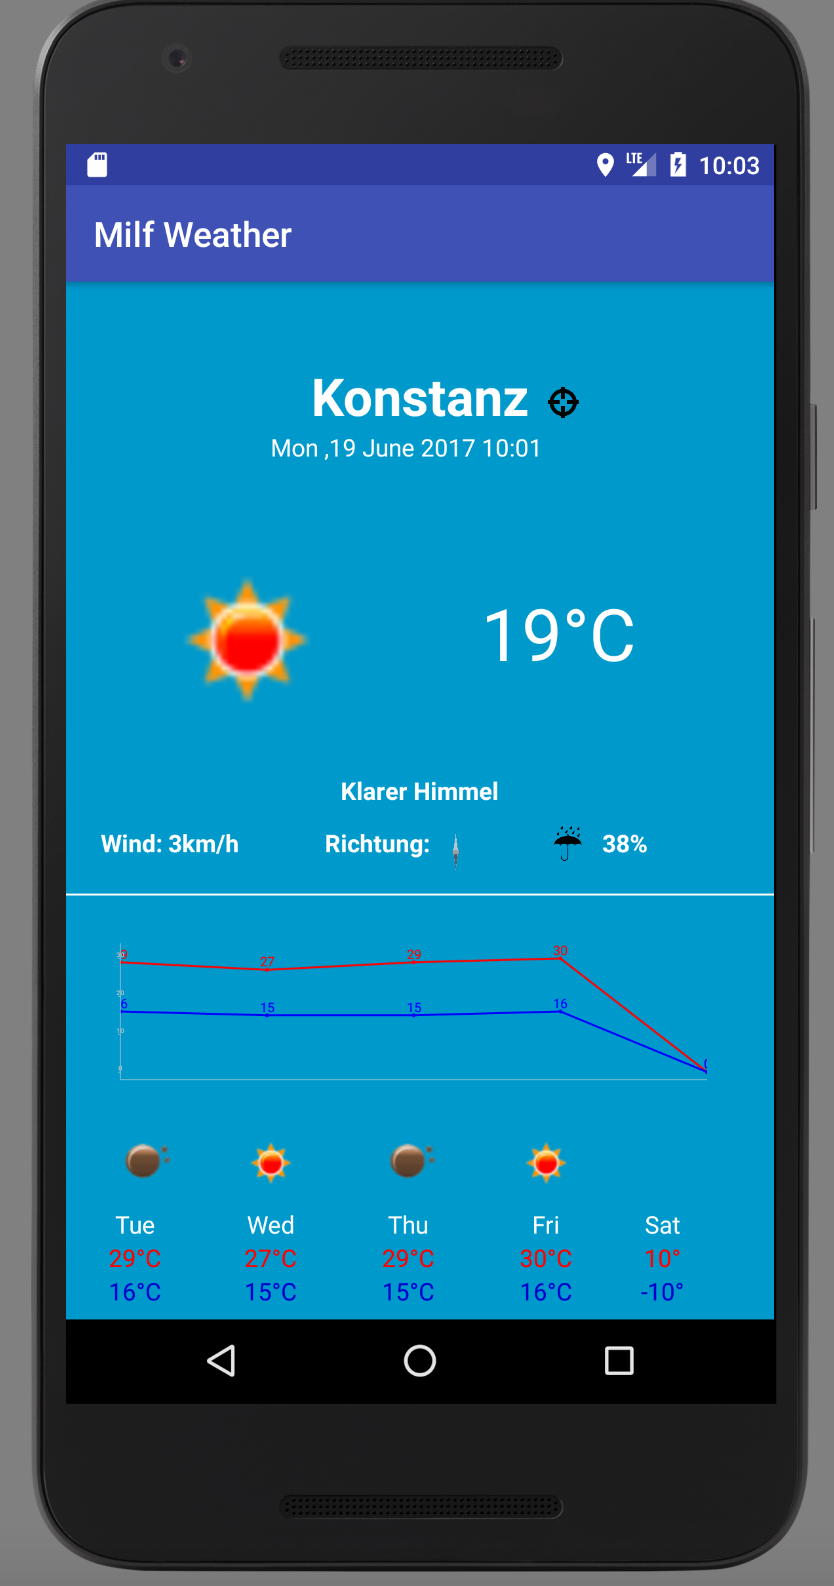
\includegraphics[width=0.5\textwidth]{Bilder/AndroidApp.png}}
    \subfigure{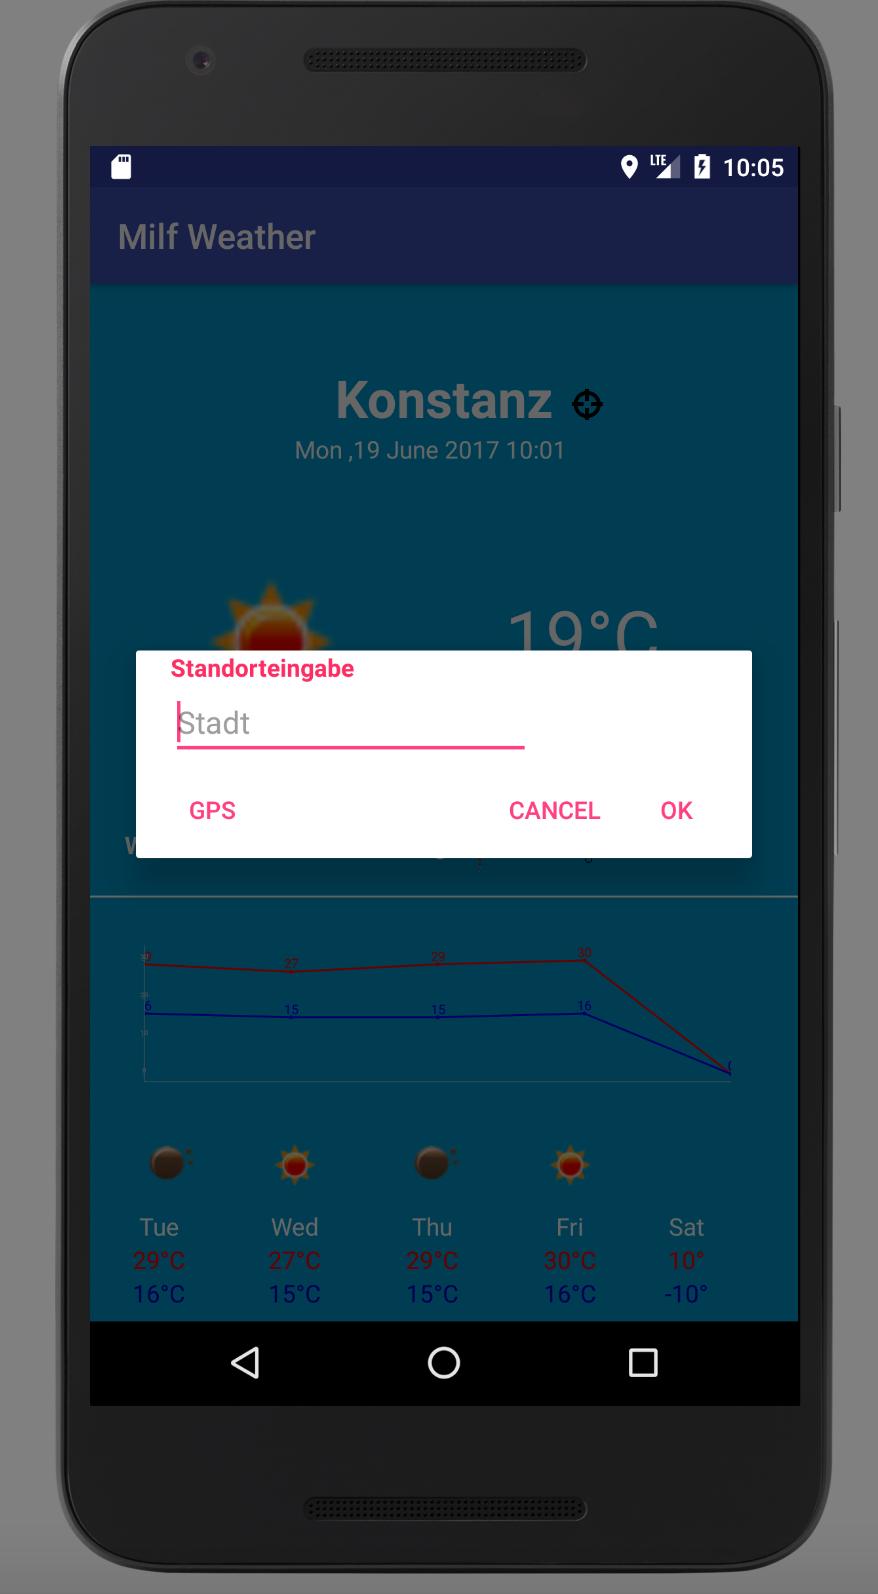
\includegraphics[width=0.5\textwidth]{Bilder/AndroidAppPLZ.png}}
\caption{Android-Applikation}
\label{img:AndroidApplikation}
\end{figure}


\subsection{Web-Client}
Zugriff direkt auf mom via Paho und mqtt-web
Zum Auslesen der env variablen php
Bootstrap Template, bootstrap für responsive design
jquery
c3.js, d3.js für den Graph
Unter deployment Kapitel: Heroku hinzufügen
